\documentclass[11pt]{article}
\usepackage[margin = 1in]{geometry}
\usepackage{amsmath}
\usepackage{amssymb}
\usepackage{amsthm}
\usepackage{graphicx}
\usepackage{subfig}
\usepackage{enumitem}
\usepackage{url}
\usepackage[parfill]{parskip}
\newcommand{\skipline}{\vspace{\baselineskip}}
\newcommand{\terminal}[1]{\text{ } <\text{#1}> \text{ }}
\newenvironment{problem}[1]{\textbf{Section #1 }}{}


\begin{document}
	
	\begin{center}
		\textbf{Homework 1} \\
		\textbf{Programming Languages} \\
		\textbf{CS 320} \\
		\textbf{Stephen Giang RedID: 823184070} \\
	\end{center}
	\skipline
	\skipline
	\begin{problem}{A.}\underline{Regular Expressions} 
		\\ \\
		Write "regex" statements for the following patterns:
		\begin{enumerate}[label = (\alph*)]
			\item A string that has either "comp" or "imp"  \\
			Expression: ".*(co$|$i)mp.*" 
			\item A string that starts and ends with "virus" \\
			Expression: "\^{}virus.*virus\$" 
			\item A string that has a "z" followed by at least one "o" \\
			Expression: "zo+" 
		\end{enumerate}
	\end{problem}
	\skipline
	\skipline
	\begin{problem}{B.}\underline{Sebesta Review Questions}
		\begin{enumerate}[label = (\alph*)]
			\item Define syntax and semantics. 
			\\ \\
			Syntax - the form or structure of the expressions, statements, and program units \\
			Semantics - the meaning of the expressions, statements, and program units
			\item Define a left-recursive grammar rule. 
			\\ \\
			Left-Recursive Grammar Rule - a rule in which the leftmost variable on the right hand side  is the same as the variable on the right hand side.
		\end{enumerate}
	\end{problem}
	\newpage
	\begin{problem}{C.}\underline{From Sebesta Problem Set Questions}
		\begin{enumerate}
			\item Write an EBNF description for a Java class definition header statement.
			\begin{align*}
				< \text{header} > &\rightarrow \text{ } <\text{modifier}> \textbf{class} <\text{class\textunderscore name}> \\
				&\text{ } [\textbf{extends} < \text{extend \textunderscore class \textunderscore name} >] \\
				&\text{ } [\textbf{implements} < \text{interface \textunderscore name} > \{, < \text{interface \textunderscore name} >\}] \\
				<\text{modifier}> &\rightarrow \text{public } | \text{ abstract } | \text{ final} 
			\end{align*}
			\newpage
			\item Using the grammar in Example 3.2, show a parse tree and a leftmost derivation for the following statement:
			\[A = A * (B + (C * A))\]
			\begin{align*}
				<\text{assign}> &\rightarrow \text{ } <\text{id}> \text{ } = \text{ }<\text{expr}> \\
				&\rightarrow \text{ A } = \text{ } <\text{expr}> \\
				&\rightarrow \text{ A } = \text{ } <\text{id}> \text{ } * \text{ } <\text{expr}> \\
				&\rightarrow \text{ A } = \text{ } \text{ A } * \text{ } <\text{expr}> \\
				&\rightarrow \text{ A } = \text{ } \text{ A } * \text{ } (<\text{expr}>) \\
				&\rightarrow \text{ A } = \text{ } \text{ A } * \text{ } (<\text{id}> \text{ } + \text{ } <\text{expr}>) \\
				&\rightarrow \text{ A } = \text{ } \text{ A } * \text{ } (B \text{ } + \text{ } <\text{expr}>) \\
				&\rightarrow \text{ A } = \text{ } \text{ A } * \text{ } (B \text{ } + \text{ } (<\text{expr}>)) \\
				&\rightarrow \text{ A } = \text{ } \text{ A } * \text{ } (B \text{ } + \text{ } (<\text{id}>\text{ }*\text{ } <\text{expr}>)) \\
				&\rightarrow \text{ A } = \text{ } \text{ A } * \text{ } (B \text{ } + \text{ } (\text{ C }*\text{ } <\text{expr}>)) \\
				&\rightarrow \text{ A } = \text{ } \text{ A } * \text{ } (B \text{ } + \text{ } (\text{ C }*\text{ } <\text{id}>)) \\
				&\rightarrow \text{ A } = \text{ } \text{ A } * \text{ } (B \text{ } + \text{ } (\text{ C }*\text{ } A)) 
			\end{align*}
			\hspace{3cm}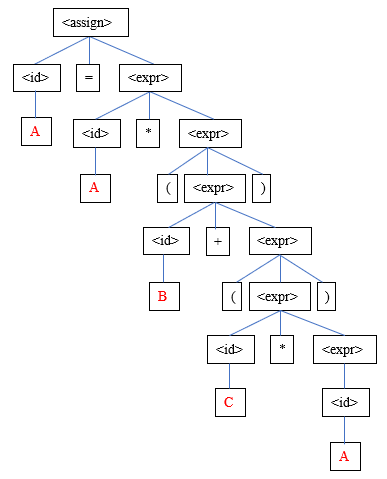
\includegraphics{ParseTree.png}
			\newpage
			\item Using the grammar in Example 3.2, show a parse tree and a leftmost derivation for the following statement:
			\[A = (A+B) * C\]
			\begin{align*}
				<\text{assign}> &\rightarrow \terminal{id} = \terminal{expr} \\
				&\rightarrow A = \terminal{expr} \\
				&\rightarrow A = \terminal{term} \\
				&\rightarrow A = \terminal{term} * \terminal{factor} \\
				&\rightarrow A = \terminal{factor} * \terminal{factor} \\
				&\rightarrow A = \text{ } (< \text{expr} >) \text{ } * \terminal{factor} \\
				&\rightarrow A = \text{ } (< \text{expr} > + \text{ } < \text{term} >) \text{ } * \terminal{factor} \\
				&\rightarrow A = \text{ } (< \text{term} > + \text{ } < \text{term} >) \text{ } * \terminal{factor} \\
				&\rightarrow A = \text{ } (< \text{factor} > + \text{ } < \text{term} >) \text{ } * \terminal{factor} \\
				&\rightarrow A = \text{ } (< \text{id} > + \text{ } < \text{term} >) \text{ } * \terminal{factor} \\
				&\rightarrow A = \text{ } (\text{A } + \text{ } < \text{term} >) \text{ } * \terminal{factor} \\
				&\rightarrow A = \text{ } (\text{A } + \text{ } < \text{factor} >) \text{ } * \terminal{factor} \\
				&\rightarrow A = \text{ } (\text{A } + \text{ } < \text{id} >) \text{ } * \terminal{factor} \\
				&\rightarrow A = \text{ } (\text{A } + \text{ B}) \text{ } * \terminal{factor} \\
				&\rightarrow A = \text{ } (\text{A } + \text{ B}) \text{ } * \terminal{id} \\
				&\rightarrow A = \text{ } (\text{A } + \text{ B}) \text{ } * \text{ C} \\
			\end{align*}
			\hspace{4cm}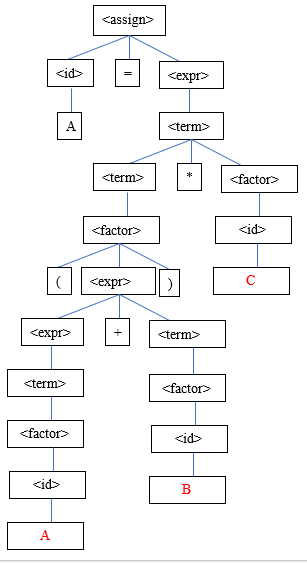
\includegraphics[height = 11cm]{ParseTree2.png}
			\newpage
			\item Consider the following grammar:
			\begin{align*}
				(S) &\rightarrow (A) \text{ } a \text{ } (B) \text{ } b \\
				(A) &\rightarrow (A) \text{ } b \text{ } | \text{ } b \\
				(B) &\rightarrow a \text{ } (B) \text{ } | \text{ } a 
			\end{align*}
			Which of the following sentences are in the language generated by this grammar?
			\begin{enumerate}[label = (\alph*)]
				\item baab 
				\begin{align*}
					(S) &\rightarrow (A) \text{ } a \text{ } (B) \text{ } b \\
					&\rightarrow b \text{ } a \text{ } (B) \text{ } b \\
					&\rightarrow b \text{ } a \text{ } a \text{ } b
				\end{align*}
				\item bbbab 
				\\
				Impossible because the conversion of $(B)$ will always give us more than one "a".
				\item bbaaaaa
				\\
				Impossible because the last letter will always be "b" in the given grammar
				\item bbaab
				\begin{align*}
					(S) &\rightarrow (A) \text{ } a \text{ } (B) \text{ } b \\
					&\rightarrow (A) \text{ } b \text{ } a \text{ } (B) \text{ } b \\
					&\rightarrow b \text{ } b \text{ } a \text{ } (B) \text{ } b \\
					&\rightarrow b \text{ } b \text{ } a \text{ } a \text{ } b
				\end{align*}
			\end{enumerate}
		\item Convert the BNF of Example 3.1 to EBNF.
		\begin{align*}
			\terminal{program} &\rightarrow \textbf{ begin} \terminal{stmt} \{; \terminal{stmt}\} \textbf{ end} \\
			\terminal{stmt} &\rightarrow \terminal{var} = \terminal{var} \{ [+ | -] \terminal{var}\} \\
			\terminal{var} &\rightarrow A \text{ } | \text{ } B \text{ } | \text{ } C
		\end{align*}
		\end{enumerate}
	\end{problem}


\end{document}
